\section{Basic Active noise cancelling system} \label{sec:BasicSystem}
This appendix will go through the different basic active noise cancelling system topologies and explain the choosen topology in detail. There are three basic different topologies for noise cancelling, feedforward, feedback and hybrid feedforward/feedback. These topologies each have their advantages and disadvantages and therefore a suitable topology must be chosen.

A general ANC system uses either one or two signals depending on the topology as input to an adaptive optimization algorithm. The inputs are used to determine coefficients for a control filter which calculates as an estimation of the transfer function from the feedforward microphone to the transducer. In an ideal case the filter would be a FIR filter with a -1 tap. This is assuming no delay or magnitude change in either the physical world or in the ANC system and no feedback from the transducer to the feedforward microphone. This is of cause not the case in reality. 




\subsection*{Feedforward}
A feedforward ANC system consists of the following as seen on \autoref{fig:feedforwardTopology}.
\begin{figure}[H]
	\centering
	\includegraphics[width=0.75\textwidth]{figures/BasicSystem/feedforward}
	\caption{Typical control system layout with on-line cancellation path identification. (Maybe switched with headphone figure)}
	\label{fig:feedforwardTopology}
\end{figure}
Where:
\begin{itemize}
\item Reference microphone: The microphone which picks up the noise to be cancelled 
\item Error microphone: The microphone which measures the the residual between the noise and the output of the ANC system
\item Control filter: Estimate of transfer function from reference microphone to transducer. 
\item Adaptive FXLMS algorithm: FXLMS optimization algorithm for the coefficients of the control filter
\item Cancellation path estimate: Impulse response from the transducer to the error microphone
\item Adaptive algorithm: LMS optimization algorithm for the coefficients of the Cancellation path estimate 
\end{itemize}

The feedforward topology uses a reference microphone to pick up the noise which is fed into the control filter which is the estimated impulse response of the path from the reference microphone to the transducer. The control filter can either be realized as a FIR filter if there is no feedback from the transducer to the reference micophone. An IIR filter should be used if there is feedback. It should be noted that if the filter is chosen to be an IIR filter there is a possibility of not getting a global minimum in the FXLMS algorithm.

The advantage of the feedforward topology is that it can cancel all types of sound. The disadvantage is that in order for the feedforward to have a good performance, the delay of the system must be less than the propagation time of the sound from the reference microphone to the transducer.    




\subsection*{Feedback}
A feedback ANC system consists of the following as seen on \autoref{fig:feedbackTopology}.
\begin{figure}[H]
	\centering
	\includegraphics[width=0.6\textwidth]{figures/BasicSystem/feedback}
	\caption{Adaptive feedback controller with on-line cancellation path identification. (Maybe switched with headphone figure)}
	\label{fig:feedbackTopology}
\end{figure}

The feedback topology uses a pseudo-reference signal synthesised from the error microphone to cancel out periodic noise. The disadvantage of the feedback topology is then that it cannot cancel out non periodic noise.    




\subsection*{Hybrid feedforward/feedback}    
A hybrid feedforward/feedback ANC system consists of the following as seen on \autoref{fig:hybridTopology}.
\begin{figure}[H]
	\centering
	\includegraphics[width=0.6\textwidth]{figures/BasicSystem/hybrid}
	\caption{Configuration for hybrid feedforward/feedback control system. (Maybe switched with headphone figure)}
	\label{fig:hybridTopology}
\end{figure}

The hybrid feedforward/feedback uses both topologies advantages to get increased performance. The topology cancels periodic noise using feedback and non periodic noise with the feedforward. The disadvantage of the hybrid topology is that the system is more advanced than the other two topologies.   

From the examination of the three different topologies it is concluded that a feedforward system will be used. The reasoning behind this choice is that the feedback system only is capable of cancelling periodic noise. The hybrid feedforward/feedbacks increased performance comes from using the feedback part to reduce periodic noise which is non existent in speech signals. With the topology chosen a system design using headphones can now be derived. 



\newpage 
\section{System Design} \label{sec:systemDesign}
This appendix will go through the design of the system using a feedforward topology. The ANC system will be placed on a headphone with the microphones placed as seen on \autoref{fig:SystemHeadphone}. A \fxnote{dummy} will be used as the HATS during tests. This means that the cancellation path will have a constant impulse response. 
\begin{figure}[H]
	\centering
	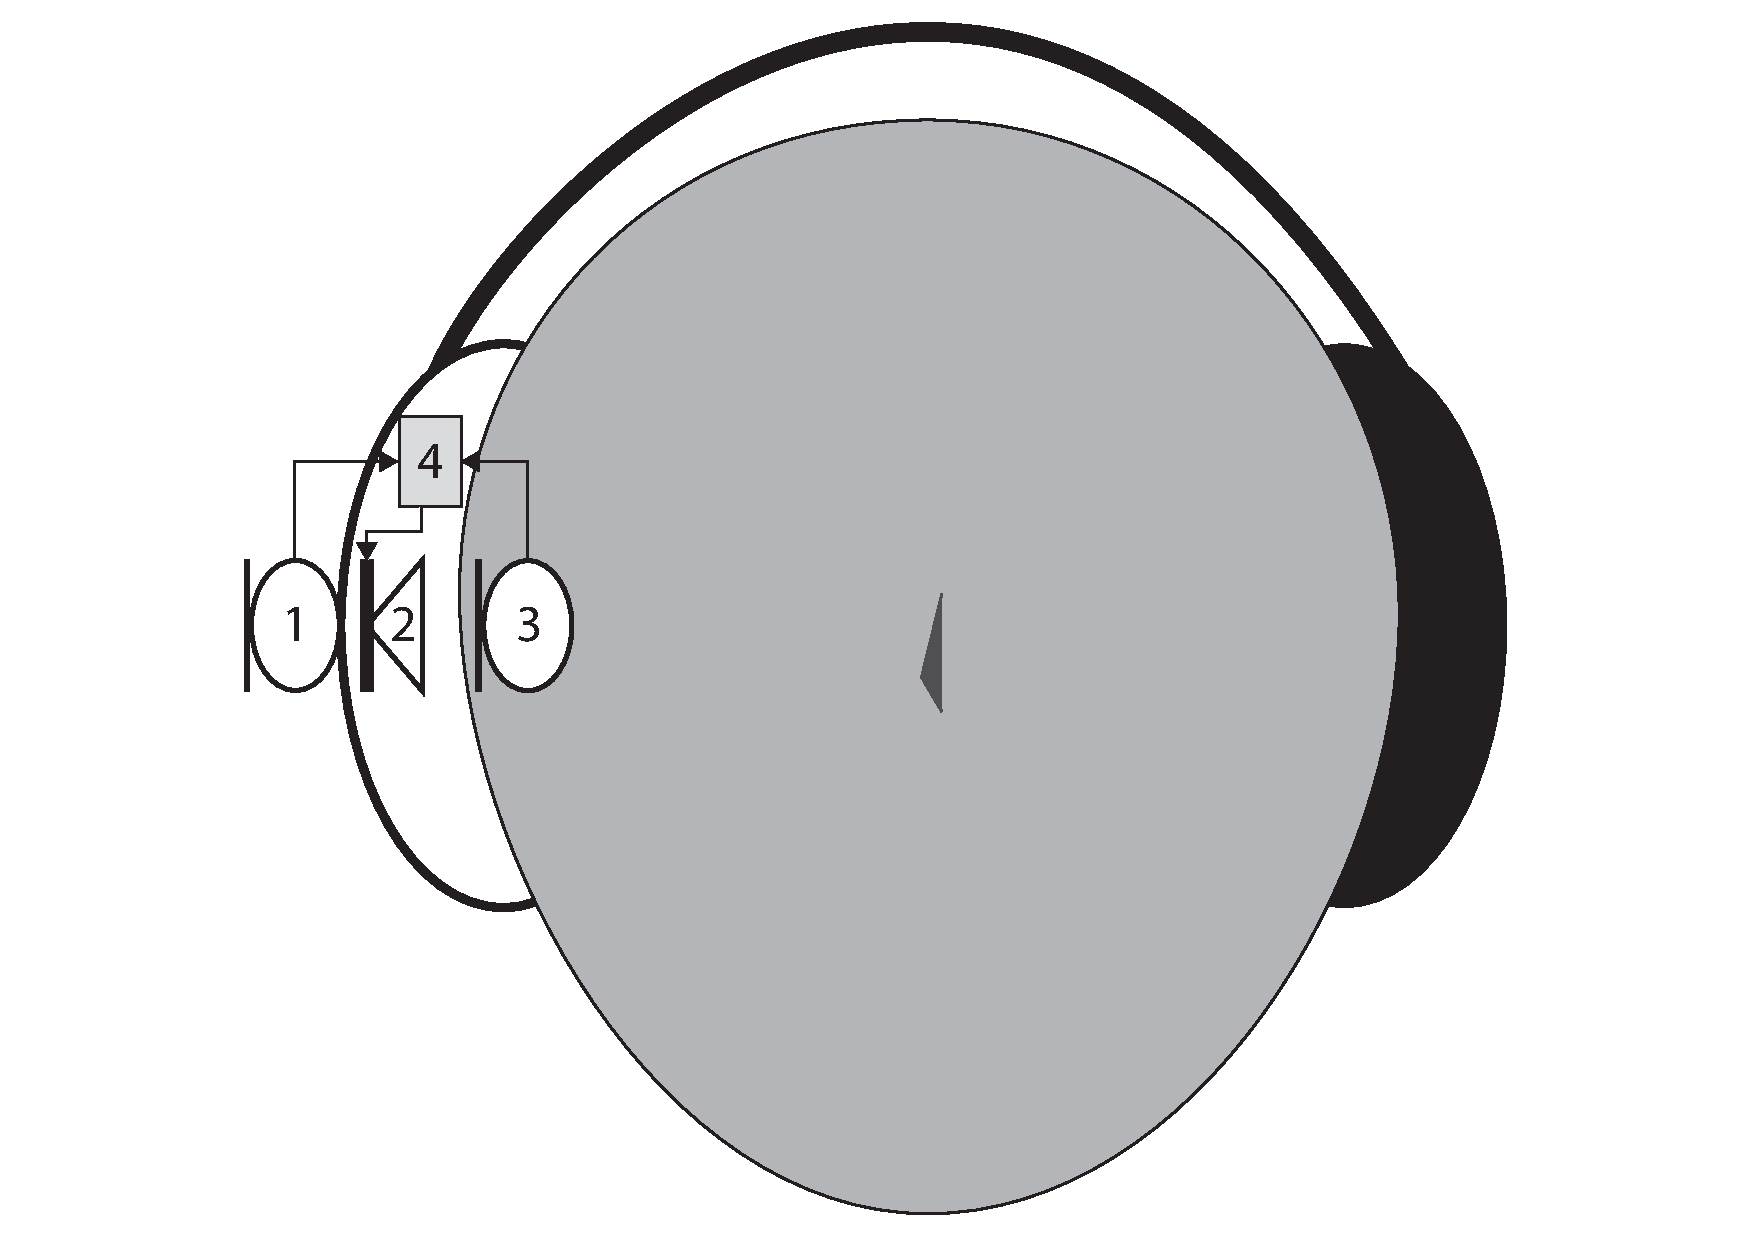
\includegraphics[width=0.6\textwidth]{ArticleIllustrations/SystemOverview}
	\caption{Headphone look}
	\label{fig:SystemHeadphone}
\end{figure}  

Because the cancellation path is constant, the adaptive algorithm adjusting the cancellation path estimate will not be in the basic system. This means that the copy of the cancellation path estimate will be a constant impulse response. The cancellation path has been found as described in \autoref{sec:CPjournal}\fxnote{Do we need to have the resulting impulse response here?}. The basic feedforward control system is seen on \autoref{fig:BasicSystem}. 

\begin{figure}[H]
	\centering
	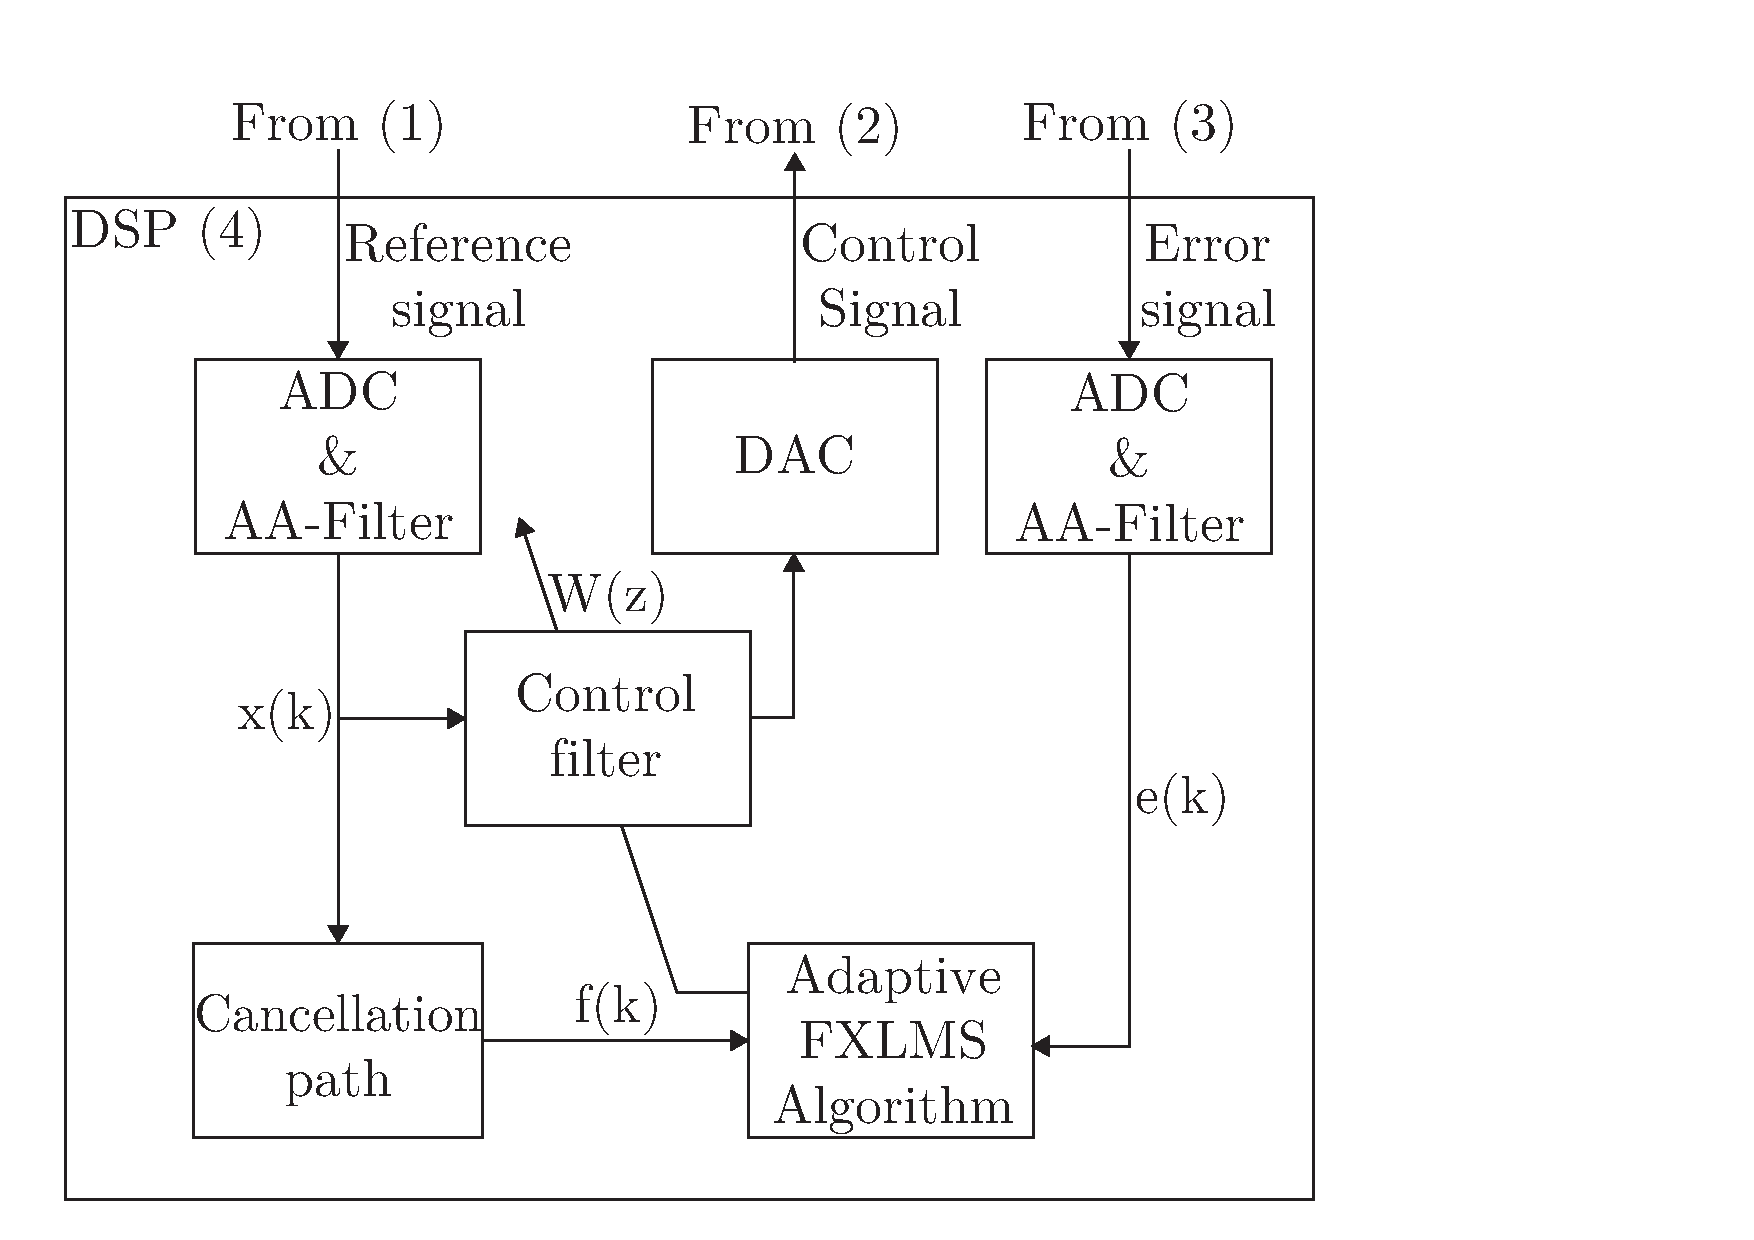
\includegraphics[width=1.0\textwidth]{ArticleIllustrations/ANCFeedForward}
	\caption{Block of basic System without adaptive CP}
	\label{fig:BasicSystem}
\end{figure}   

\fxnote{Possibly missing text}





\subsection{FXLMS algorithm for FIR filters}\label{subsec:fxlms}
The FXLMS is a gradient descent algorithm which iteratively changes the coefficients of the control filter by adding a calculated step to the current coefficients which should converge to a global minimum of the error criterion. The derivation of the FXLMS algorithm is given below. 
\begin{equation}\label{eq:FXLMSNewCoef}
w(k+1) = w(k) - \mu\nabla J(k)
\end{equation}
Where:
\begin{description}
	\item[\text{$\nabla$J}] is the gradient of the error surface at the location given by the current weight coefficient
	\item[\text{$\mu$}] is a convergence factor
	\item[w(k)] is the weight coefficients of the control filter written as  $w(k)=[w_(k),w_1(k) \cdots w_{L-1}(k)]^T$
\end{description}
The error is defined as:
\begin{equation}\label{eq:FXLMSError}
e(k) = p(k) + s(k)
\end{equation}
Where:
\begin{description}
	\item[\text{$p(k)$}] is the primary noise source
	\item[\text{$s(k)$}] is the control source
\end{description}

The error criterion as a function of the filter weights is to be minimized therefore the gradient of the error surface ($\nabla J$) is calculated by differentiating the mean squared error, as shown in equation \ref{eq:FXLMSGradient} 
\begin{equation}\label{eq:FXLMSGradient}
J(k) = e^2(k)
\end{equation}

Differentiating equation \ref{eq:FXLMSGradient} with respect to $w(k)$ yields equation \ref{eq:FXLMSGradientW(k)}. The last substitution can be made because $p(k)$ does not depend on $w(k)$. So the term $p(k)$ from equation \ref{eq:FXLMSError} does not influence the gradient of $e(k)$:

\begin{equation}\label{eq:FXLMSGradientW(k)}
\Delta w(k) = \frac{\partial e^2(k)}{\partial w(k)} = 2e(k)\frac{\partial e(k)}{\partial w(k)} = 2e(k)\frac{\partial s(k)}{\partial w(k)}
\end{equation}
$e(k)$ can be sampled. How to obtain s(k) is described below. \\
The controller output signal y(k) is given by equation \ref{eq:FXLMSOutput} 

\begin{equation}\label{eq:FXLMSOutput}
y(k) = w^T(k) + x(k) = \sum_{i=0}^{L-1} w_i(k)x(k-i)
\end{equation}
Where:
\begin{description}
	\item[x(k)] = $[x(k) x(k-1) \cdots x(k-L+1)]^T $
\end{description}
$s(k)$ can be formulated as equation \ref{eq:FXLMSs(k)}

\begin{equation}\label{eq:FXLMSs(k)}
s(k) = [w^T(k)x(k)]*c(k)\approx y(k)*\hat{c}(k) = \sum_{i=0}^{M-1}\hat{c}_i(k)y(k-1)
\end{equation}
Where:
\begin{description}
	\item[y(k)] = $[ y(k) y(k-1) \cdots y(k-M+1)]$
	\item[c(k)] is the impulse response of the cancellation path (The Taps)
\end{description}

Equation \ref{eq:FXLMSs(k)} can be rewritten to equation \ref{eq:FXLMSs(k)2}

\begin{equation}\label{eq:FXLMSs(k)2}
s(k) = [w^T(k)x(k)]*c(k)\approx w^T(k)*f(k)
\end{equation}
Where:
\begin{description}
	\item[f(k)] is the filtered reference signal $f(k)=x(k)c(k)$
	\item[f(k-j)] = $\sum_{i=0}^{M-1}\hat{c}_i(k)x(k-i-j)$
\end{description}

By using equation \ref{eq:FXLMSs(k)2} in substituting into equation \ref{eq:FXLMSGradientW(k)}, the error of the surface gradient can be written as equation \ref{eq:FXLMSNablaJ}.

\begin{equation}\label{eq:FXLMSNablaJ}
\nabla J = 2e(k)\frac{\partial s(k)}{\partial w(k)} = 2e(k)f(k)
\end{equation}

Which yields equation \ref{eq:FXLMSw(k+1)}

\begin{equation}\label{eq:FXLMSw(k+1)}
w(k+1) = w(k) - 2\mu e(k)f(k)
\end{equation}

Which is the standard FXLMS algorithm using an adaptive FIR filter
\begin{equation}\label{eq:FXLMSw_j(k+1)}
w_j(k+1) = w_k(k) - 2\mu e(k)f(k-j)
\end{equation}

With the definition of the FXLMS given the basic system in \autoref{fig:BasicSystem}, can be simulated.







\subsection{Simulation} 
The basic system in \autoref{fig:BasicSystem} has been setup in Simulink, as seen on \autoref{fig:SimulinkRealWorld} which resembles the real world and \autoref{fig:SimulinkANC} which resembles the ANC algorithm on a dsp. 

\begin{figure}[H]
	\centering
	\includegraphics[width=1\textwidth]{figures/BasicSystem/SimulinkRealWorld}
	\caption{Simulink real world.}
	\label{fig:SimulinkRealWorld}
\end{figure}    

\begin{figure}[H]
	\centering
	\includegraphics[width=1\textwidth]{figures/BasicSystem/SimulinkANC}
	\caption{Simulink ANC algorithm}
	\label{fig:SimulinkANC}
\end{figure} 

The functions for the different impulse responses and the control filter is a standard sample-by-sample FIR filter, while the FXLMS algorithm is \autoref{eq:FXLMSw_j(k+1)} implemented with a convergence factor of 0.005. The delay of the ADC and DAC is set to 0 samples.\fxnote{Which results do we need}



